\documentclass{beamer}
\usetheme{Ilmenau}
\usecolortheme{default}
\usefonttheme{serif}

\usepackage{lipsum}
\usepackage{graphicx,xcolor,tikz,pgfplots}
\pgfplotsset{compat=1.14}
\usepackage{amsmath,amssymb,amsfonts}
\usetikzlibrary[automata] % ConTEXt
\usepackage{rotating}
\usepackage[export]{adjustbox}
\usepackage{relsize}
\tikzset{fontscale/.style = {font=\relsize{#1}}
    }

\newtheorem{thm}{Theorem}
\newtheorem{dfn}{Definition}

\newcommand{\ds}{\displaystyle}
\newcommand{\R}{{\mathbb R}}
\newcommand{\Q}{{\mathbb Q}}
\newcommand{\Z}{{\mathbb Z}}
\newcommand{\N}{{\mathbb N}}
\newcommand{\C}{{\mathbb C}}
\DeclareMathOperator{\Ap}{Ap}
\DeclareMathOperator{\PF}{PF}
\DeclareMathOperator{\KC}{KC}
\DeclareMathOperator{\ewt}{ewt}
\DeclareMathOperator{\wt}{wt}

\setbeamertemplate{footline}[frame number]{}
\setbeamertemplate{navigation symbols}{}

\defbeamertemplate*{headline}{split theme}
{}


\title{Pflueger's Conjecture for Numerical Semigroups of Small Depths\\[5pt]\footnotesize{\textit{Math Club GAUSS Talk}}}
\author{Ian Farish, Erik Imathiu-Jones, Kaylee Seojin Lee Kim, Max LaFortune, Cole McGeorge, \textbf{Victoria Wiest}
\\[15pt] Graduate Student Advisors: Fabian Ramirez, Deepesh Singhal
\\[15pt] Faculty Advisor: Dr. Nathan Kaplan}
\institute{}
\date{}

\begin{document}

\begin{frame}
\titlepage
\end{frame}

\section{Preliminaries}
\begin{frame}{Numerical Semigroups}
    A nonempty subset of $\N_{0}=\{0,1,2,3,\dots\}$, denoted as $S$, is a \textbf{numerical semigroup}, if and only if

    \begin{itemize}
        \item $0\in S$,
        \item $\N_{0} - S$ is finite, and
        \item If $x\in S$ and $y\in S$, then $x+y\in S$ (closed under addition)
    \end{itemize}\vspace{8pt}
    Ex: $\{0,3,4,6,7,8,\to\}$
    
\end{frame}

\begin{frame}{Definitions related to Numerical Semigroups}
    The smallest nonzero element in $S$ is called the \textbf{multiplicity}, denoted by $m(S)$.\\[15pt]
    
    We refer to $\N_{0} - S$ as the set of gaps in the numerical semigroup. 
    \begin{itemize}
        \item The number of gaps of a numerical semigroup is called the \textbf{genus}, denoted as $g(S).$
        \item The \textbf{Frobenius number}, $F(S)$, of a numerical semigroup is the largest gap.
    \end{itemize}
    \vspace{15pt}
    The \textbf{depth} of a numerical semigroup $S$ is the natural number $d$ such that 
    \[(d-1)m<F<dm.\]
\end{frame}

\begin{frame}{Minimal Generators}
    Every numerical semigroup, $S$, has a unique \textbf{minimal generating set} that generates $S$ by taking all possible sums of the numbers in the minimal generating set i.e., 
    \[\langle3,4\rangle=\{0,3,4,3+3,3+4,4+4,\to\}=\{0,3,4,6,7,8,\to\}\]\\[15pt]
    
    We refer to the elements in the minimal generating set as \textbf{minimal generators}.
\end{frame}

\begin{frame}{Young Diagram associated to a NS}
Every numerical semigroup is associated to some Young Diagram where \textbf{every element in $S$ is represented as a right step} ($\rightarrow$) and \textbf{every gap is represented as an up step} ($\uparrow$).\\[15pt]

    Ex: $\langle 3,8,10\rangle=\{0,3,6,8,9,10,\to\}$

        \begin{center}
            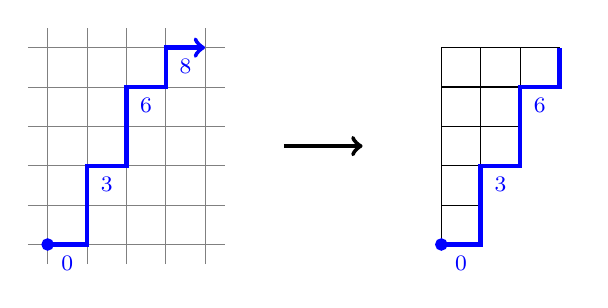
\begin{tikzpicture}[scale = .5]
		
			% 1 - rim lines
			\begin{scope}
				\draw[help lines] (-.5,-.5) grid (4.5,5.5);
				
				\begin{scope}[blue, ultra thick]
					\filldraw (0,0) circle [radius = 0.1];
					\draw[->, font = \footnotesize]
						(0,0) --
						node [below] {$0$} ++(1,0) --
						node [right] {} ++(0,1) -- 
						node [right] {} ++(0,1) --
						node [below] {$3$} ++(1,0) --
						node [right] {} ++(0,1) --
						node [right] {} ++(0,1) --
						node [below] {$6$} ++(1,0) --
						node [right] {} ++(0,1) --
						node [below] {$8$} ++(1,0);
				\end{scope}
			\end{scope}
		
			% 2 - rim with Young diagram and hooks
			\begin{scope}[xshift = 10cm]
                \foreach \x in {0,1,2}
					{ \draw (\x,4) rectangle ++(1,1);}
                \foreach \x in {0,1}
					{ \draw (\x,3) rectangle ++(1,1);}
				\foreach \x in {0,1}
					{ \draw (\x,2) rectangle ++(1,1);}
				\foreach \x in {0}
					{ \draw (\x,1) rectangle ++(1,1);}
				\foreach \x in {0}
					{ \draw (\x,0) rectangle ++(1,1);}
				
				\begin{scope}[blue, ultra thick]
					\filldraw (0,0) circle [radius = 0.1];
					\draw[font = \footnotesize]
						(0,0) --
						node [below] {$0$} ++(1,0) --
						node [right] {} ++(0,1) -- 
						node [right] {} ++(0,1) --
						node [below] {$3$} ++(1,0) --
						node [right] {} ++(0,1) --
						node [right] {} ++(0,1) --
						node [below] {$6$} ++(1,0) --
      					node [right] {} ++(0,1);
				\end{scope}
			\end{scope}
			
			
			% arrows
			\begin{scope}[ultra thick,  black, ->]
				\draw (6,2.5) -- (8,2.5);
				%\draw (13,2.5) -- (15,2.5);
			\end{scope}
		\end{tikzpicture}
        \end{center}    
\end{frame}

\begin{frame}{Weight}
    The \textbf{weight} of a numerical semigroup $S$, denoted by $\wt(S)$, is
    \[\sum_{x\in S} \#\{\text{gaps above}\; x\}\quad\text{where}\; x>0\]

    Ex: $\langle3,8,10\rangle=\{0,3,6,8,\to\}$
    \begin{center}
        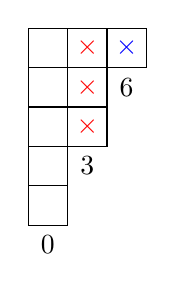
\begin{tikzpicture}[scale=0.5]
            \begin{scope}[xshift = 16cm]
                \foreach \x in {0,1,2}
					{ \draw (\x,4) rectangle ++(1,1);}
                \foreach \x in {0,1}
					{ \draw (\x,3) rectangle ++(1,1);}
				\foreach \x in {0,1}
					{ \draw (\x,2) rectangle ++(1,1);}
				\foreach \x in {0}
					{ \draw (\x,1) rectangle ++(1,1);}
				\foreach \x in {0}
					{ \draw (\x,0) rectangle ++(1,1);}
            \begin{scope}
                    \node at (0.5,-0.5) {$0$};
					\node at (1.5,1.5) {$3$};
					\node at (2.5,3.5) {$6$};
			\end{scope}
            \begin{scope}[red]
				\node at (1.5,2.5) {$\times$};
    			\node at (1.5,3.5) {$\times$};
				\node at (1.5,4.5) {$\times$};

            \end{scope}
            \begin{scope}[blue]
                \node at (2.5,4.5) {$\times$};
            \end{scope}
   		\end{scope}

        \end{tikzpicture}
    \end{center}
    \[\wt=4\]

\end{frame}

\begin{frame}{Upper Bound of Weight}
    \[S=\langle 2,2g+1\rangle\]

    \hfill

    \begin{center}
        \begin{tikzpicture}[scale=2]
            \coordinate (A) at (0,0);
            \coordinate (B) at (0.5,0);
            \coordinate (C) at (0.5,0.5);
            \coordinate (D) at (1,0.5);
            \coordinate (E) at (1,1);
            \coordinate (F) at (1.5,1);
            \coordinate (G) at (1.5,1.5);
            \coordinate (H) at (2,1.5);
            \coordinate (I) at (2,2);
            \coordinate (J) at (2.5,2);
            \coordinate (K) at (2.5,2.5);
            \coordinate (L) at (0,2.5);
            \coordinate (M) at (0.5,2.5);
            

            \draw (A) -- (B);
            \draw (B) -- (C);
            \draw (C) -- (D);
            \draw (D) -- (E);
            \draw (E) -- (F);
            \draw (F) -- (G);
            \draw (G) -- (H);
            \draw (H) -- (I);
            \draw (I) -- (J);
            \draw (J) -- (K);
            \draw (K) -- (L);
            \draw (L) -- (A);
            \draw (M) -- (B);

            \draw[decorate,decoration={brace,amplitude=3mm, raise=0.5mm}] (A) -- (L);

            \node at (-0.4,1.25) {$g$};
            \node at (1.15,1.7) [fontscale=3.45] {$\frac{g(g-1)}{2}$};
            \node at (0.25,-0.15) {$0$};
            \node at (0.75,0.35) {$2$};
        \end{tikzpicture}
        \end{center}    
\end{frame}

\begin{frame}{Effective Weight}
    Similar to the weight of a numerical semigroup, the \textbf{effective weight} of a numerical semigroup $S$, denoted by $\ewt(S)$, is
    \[\sum_{x\in S} \#\{\text{gaps above}\; x\}\quad\text{where}\; x\;\text{is a minimal generator}\]

    Ex: $\langle3,8,10\rangle=\{0,3,6,8,\to\}$    

    \begin{center}
        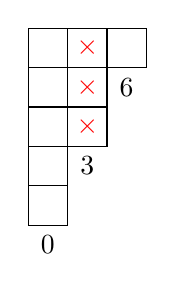
\begin{tikzpicture}[scale=0.5]
            \begin{scope}[xshift = 16cm]
                \foreach \x in {0,1,2}
					{ \draw (\x,4) rectangle ++(1,1);}
                \foreach \x in {0,1}
					{ \draw (\x,3) rectangle ++(1,1);}
				\foreach \x in {0,1}
					{ \draw (\x,2) rectangle ++(1,1);}
				\foreach \x in {0}
					{ \draw (\x,1) rectangle ++(1,1);}
				\foreach \x in {0}
					{ \draw (\x,0) rectangle ++(1,1);}
            \begin{scope}
                    \node at (0.5,-0.5) {$0$};
					\node at (1.5,1.5) {$3$};
					\node at (2.5,3.5) {$6$};
			\end{scope}
            \begin{scope}[red]
				\node at (1.5,2.5) {$\times$};
    			\node at (1.5,3.5) {$\times$};
				\node at (1.5,4.5) {$\times$};

            \end{scope}
   		\end{scope}

        \end{tikzpicture}
    \end{center}
    
    \[\ewt=3\]
\end{frame}

\begin{frame}{Pflueger's Conjecture}
    Analogously to the upper bound of $\wt(S)$, Nathan Plueger [1] has conjectured the following upper bound of $\ewt(S)$:
  \[\ewt(S)\leq\left\lfloor\frac{(g+1)^2}{8} \right\rfloor\]

  But unlike the upper bound of $\wt(S)$, Pflueger's upper bound has not been proven.
\end{frame}

\begin{frame}{Pflueger's Conjecture for NS of Depth 2}
    \textbf{Remember}: A numerical semigroups has depth 2 if
    \[m<F<2m\]
    where $m$ is the multiplicity and $F$ is the Frobenius number.
\end{frame}

\begin{frame}{Pflueger's Conjecture for NS of Depth 2}
    \[S=\langle m,\dots,m+k\rangle\]
    
    \hfill
    
    \begin{center}
        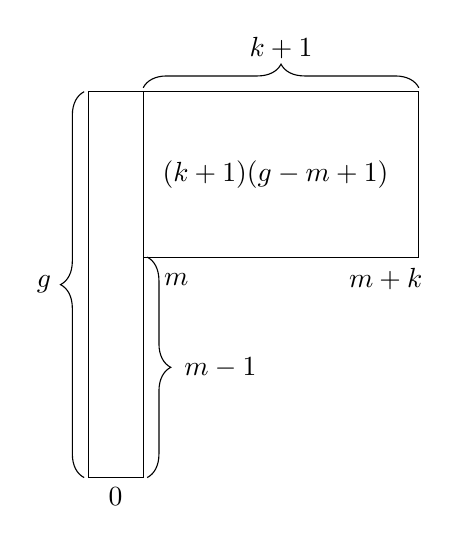
\begin{tikzpicture}[scale=1.4]
            \coordinate (A) at (0,0);
            \coordinate (B) at (0.5,2);
            \coordinate (C) at (0,3.5);
            \coordinate (D) at (0.5,0);
            \coordinate (E) at (0.5,3.5);
            \coordinate (F) at (3,2);
            \coordinate (G) at (3,3.5);
            \coordinate (H) at (0.23,1);

            \draw (A) -- (C);
            \draw (A) -- (D) node[midway, below] {$0$};
            \draw (D) -- (E);
            \draw (B) -- (E);
            \draw (B) -- (F);
            \draw (F) -- (G);
            \draw (G) -- (C);

            \node at (1.7,2.75) {$(k+1)(g-m+1)$};
            \node at (0.8,1.8) {$m$};
            \node at (2.7,1.8) {$m+k$};

            \draw[decorate,decoration={brace,amplitude=3mm, raise=0.5mm}] (A) -- (C);
            \draw[decorate,decoration={brace,amplitude=3mm, raise=0.5mm}] (B) -- (D);
            \draw[decorate,decoration={brace,amplitude=3mm, raise=0.5mm}] (E) -- (G);

            \node at (-0.4,1.75) {$g$};
            \node at (1.2,1) {$m-1$};
            \node at (1.75,3.9) {$k+1$};
        \end{tikzpicture}
        \end{center}
\end{frame}

\begin{frame}{Further Work}
    \begin{itemize}
        \item Proving Pflueger's Conjecture for numerical semigroups with larger depths (depth 3, depth 4, etc.) using Apery tuples
    \end{itemize}
\end{frame}

\section{Acknowledgments}
\begin{frame}{Acknowledgments}
Thank you to everyone on my team, including my fellow undergraduate researchers, our graduate student advisors, and our faculty advisor, Dr. Nathan Kaplan! Thank you to Cal-Bridge for their generous funding!
\begin{columns}[c]
            \begin{column}{.25\textwidth}
            \begin{figure}
                \centering
                \includegraphics[width=1\textwidth]{Victoria/Logos/CSU,Fresno.png}
            \end{figure}      
            \end{column}
            \begin{column}{.25\textwidth}
            \begin{figure}
                \centering
                \includegraphics[width=1.2\textwidth]{Victoria/Logos/Cal-Bridge.jpg}
            \end{figure}
            \end{column}
            \begin{column}{.25\textwidth}
            \begin{figure}
                \centering
                \includegraphics[width=1\textwidth]{Victoria/Logos/UC, Irvine.png}
            \end{figure}
            \end{column}
        \end{columns}

\end{frame}

\end{document}
